%!TEX program = xelatex
\documentclass[10pt]{beamer}

\usetheme[progressbar=frametitle, noframetitleoffset, block=fill]{m}
%\definecolor{TUMblue}{RGB}{55,55,255}
%\setbeamercolor{alerted text}{fg=TUMblue}

\usepackage{booktabs}
\usepackage[scale=2]{ccicons}

\usepackage{pgfplots}
\usepackage{tikz}
\usepgfplotslibrary{dateplot}
\usepackage{caption}

\newlength\figureheight
\newlength\figurewidth
\DeclareMathOperator{\prox}{prox}
\DeclareMathOperator{\argmin}{argmin}

\title{Stochastic Optimization in Machine Learning}
\subtitle{Case Studies in Nonlinear Optimization}
\date{\today}
\author{F. Bauer \and S. Chambon \and R. Halbig \and S. Heidekrüger \and J. Heuke}
\institute{Technische Universität München}
%\titlegraphic{\hfill
\includegraphics[height=1.5cm]{logo.eps}}

\begin{document}

\maketitle

\plain{
  \begin{quote}
    We're not running out of data anytime soon. It's maybe the only resource that grows exponentially.
    \\
    \flushright{\alert{Andreas Weigend}}
  \end{quote}
  }


\begin{frame}
  \frametitle{Outline}
  \setbeamertemplate{section in toc}[sections numbered]
  \tableofcontents[hideallsubsections]
\end{frame}

\section{Introduction}

  \begin{frame}[t]\frametitle{Introduction: What is Machine Learning?}
	  	Implementation of autonomously learning software for:
        \begin{itemize}
        	\item Discovery of patterns and relationships in data
        	\item Prediction of future events
        \end{itemize}
        \vspace{5pt}
        \alert{Examples:}
        \begin{columns}
        	\begin{column}{.5\linewidth}
        		Electroence-phalography (EEG)\\
        		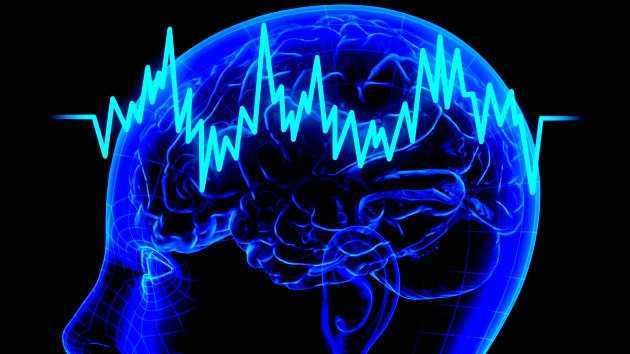
\includegraphics[width = 0.8\linewidth]{eeg_pic.jpg}\\
        		\alert{Section 4}
        	\end{column}\hspace{-10pt}
        	\begin{column}{.5\linewidth}
        		Image Denoising\\
        		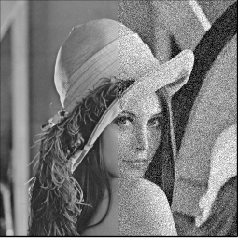
\includegraphics[width = 0.8\linewidth]{lena_pic.jpg}\\
        		\alert{Section 5}
        	\end{column}
        \end{columns}
  \end{frame}

  \begin{frame}\frametitle{ML and Optimization I}
    \alert{Training} a Machine Learning model means finding optimal parameters $\omega$:

    $$ \omega^* = \argmin_{\omega} F(\omega, X, z)$$
    \pause
    \begin{itemize}
      \item \alert{$F$}: Loss function of chosen ML-model
      \item \alert{$X$}: The training data ($N:=\#$samples $\times$ $\#$features matrix)
      \item \alert{$z$}: Training labels (only in classification models; vector of size $N$)
      \pause
      \item The dimension $n$ of $\omega$ is model dependent, often $\#$features$+1$
    \end{itemize}   
  \end{frame}

  \begin{frame}\frametitle{ML and Optimization II}
    After we have found $\omega^*$, we can do \alert{Prediction} on new data points:

    $$ \hat {z_i} := h(\omega^*, x_i)$$
    \pause
    \begin{itemize}
      \item \alert{$x_i$}: new data point with \emph{unknown} label \alert{$z_i$}
      \item \alert{$h$}: hypothesis function of the ML model
    \end{itemize}   
  \end{frame}

  \begin{frame}
    \frametitle{Challenges in Machine Learning}
      \begin{itemize}
        \item Massive amounts of training data 
        \item Construction of very large models
        \item Handling high memory/computational demands
      \end{itemize}
      \vspace{36pt}
      \pause
    \centering \large{Ansatz: \alert{Stochastic Methods}}
  \end{frame}
  
  \begin{frame}{Stochastic Framework}
    $$ F(\omega) := \mathbb{E}\left[f(\omega, \xi)\right] \uncover<3>{= \frac{1}{N}\sum_{i=1}^N f(\omega, x_i, z_i)}$$
    \begin{itemize}
      \item<2-> \alert{$\xi$}: Random variable; takes the form of an input-output-pair $(x_i, z_i)$
      \item<3-> \alert{$f$}: Partial loss function corresponding to a single data point.
    \end{itemize}
  \end{frame}

  \begin{frame}{Stochastic Methods}
    \begin{columns}[T]
      \begin{column}{.5\textwidth}
        \centering \alert{Gradient Method}
        $$\min F(\omega) $$

        \uncover<2->{
        $$\omega^{(k+1)}:= \omega^{(k)}-\alpha_k \nabla F(\omega^{(k)})$$\\
        \phantom{zeile}
        }
      \end{column}\hfill
      \begin{column}{.5\textwidth}
        \centering \alert{Stochastic Gradient Descent}
        $$\min \mathbb E \left [f(\omega, \xi)\right]$$
        \uncover<3>{
          $$\omega^{(k+1)}:= \omega^{(k)}-\alpha_k \alert{\nabla \hat F(\omega^{(k)})} $$
          with
          $$\alert{\nabla \hat F(\omega^{(k)})} := \frac{1}{b}\sum_{i\in \mathcal S_k}f(\omega, x_i, z_i)$$
          where $\mathcal S_k \subset [N], \quad b:=|\mathcal S_k| \ll N$\\\alert{"Mini Batch"}
        }
      \end{column}
    \end{columns}
  \end{frame}

\section{SQN: A Stochastic Quasi-Newton Method}

  \begin{frame}
    \frametitle{Higgs-Boson classification problem}
      \begin{itemize}
        \item Data from Monte-Carlo simulations
        \item $X\in \mathbb R^{11.000.000 \times 29}$\\\emph{Lots} of samples, relatively small, dense feature set.
        \item Here, we use \emph{Logistic Regression} for classification.
      \end{itemize}
  \end{frame}

  \begin{frame}\frametitle{Stochastic Quasi-Newton Method (SQN)}
      \begin{itemize}
        \item \alert{Stochastically} use second-order information
        \item Based on BFGS-method.
        \pause
        \item Basic idea: $$ \omega^{(k+1)} = \omega^{(k)} - \alpha_k \alert{H_t} \nabla \hat F(\omega^{(k)})$$
        \pause
        \item $t$ running on slower time-scale than $k$. 
        \item $H_t$ update in $\mathcal O(n)$ time and constant memory, using several tricks
      \end{itemize}
  \end{frame}


  \begin{frame}
    \frametitle{Behavior}
      Pretty picures about the behaviour of SQN on HIGGS
      and comparison with traditional SGD
  \end{frame}

  \begin{frame}\frametitle{Results}
    \begin{itemize}
      \item Can be faster than SGD on appropriate Datasets
      \item Requires tedious, manual tuning of hyperparameters to be efficient!
    \end{itemize}
  
  \end{frame}

 \section{Proximal Method}

   \begin{frame}{Proximal Method}
       \begin{flalign*}
       	\text{\alert{Problem}}&&
       	\min_x &\;F(x) := \underbrace{f(x)}_{smooth} \quad + \underbrace{h(x)}_{non-smooth}&
       \end{flalign*}
       \pause
       \begin{flalign*}
       	\text{\alert{Proximity Operator}}&&\prox_f(v) = &\underset{x}{\argmin} \; \bigl( f(x) + \frac{1}{2} \lVert x - v \rVert^2_2 \bigr)&
       \end{flalign*}
			\centering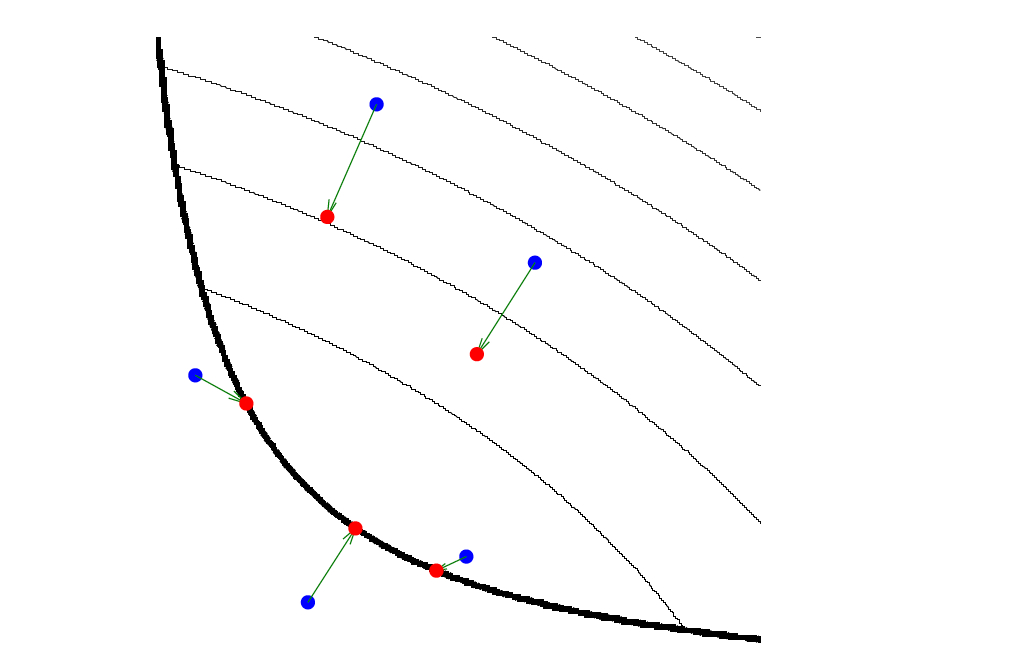
\includegraphics[width = 0.5\textwidth]{prox_boyd.jpg}
   \end{frame}
   
   \begin{frame}{Proximal Method}
   	\alert{Traditional Proximal Gradient Step:}
   	\begin{equation*}
   	x_{k+1} = \prox_{\lambda_kh}(x_k - \lambda_k\nabla f(x_k))
   	\end{equation*}
   	\alert{Quasi-Newton Proximal Step:}
   	\begin{equation*}
   	x_{k+1} = \prox_h^{B_k}(x_k - B_k^{-1}\nabla f(x_k)),
   	\end{equation*}
   	with $B_k = \underbrace{D_k}_{diag} + \underbrace{u_k}_{\in\mathbb{R}^n}u_k^T$.
   \end{frame}
   
   \begin{frame}{Proximal Method}
   	\begin{columns}[T]
   		\begin{column}{.5\textwidth}
   			$F(x) = \lVert Ax - b \rVert + \lambda \lVert x \rVert_1$\\
   			$A \in \mathbb{R}^{1500 \times 3000},\:b \in \mathbb{R}^{1500}$\\
   			$A_{ij},\:b_i\:$ \textasciitilde $\:\mathcal{N}(0,1)$, $\:\lambda = 0.1$\\
   			\vspace{28pt}
   			\resizebox{\linewidth}{!}{% This file was created by matplotlib v0.1.0.
% Copyright (c) 2010--2014, Nico Schl�mer <nico.schloemer@gmail.com>
% All rights reserved.
% 
% The lastest updates can be retrieved from
% 
% https://github.com/nschloe/matplotlib2tikz
% 
% where you can also submit bug reports and leavecomments.
% 
\begin{tikzpicture}

\begin{axis}[
xlabel={Number of Iterations},
ylabel={Function Value},
xmin=0, xmax=55,
ymin=10, ymax=10000000000000,
ymode=log,
axis on top,
legend entries={{0SR1},{ProxGrad},{L-BFGS-B}}
]
\addplot [thick, red]
coordinates {
(0,23930.000884189)
(1,2334714540827.73)
(2,1603.06839363472)
(3,1004.45275331694)
(4,588.495767390219)
(5,2465.40475724742)
(6,179.594821649387)
(7,126.10021752328)
(8,61.4875604431263)
(9,129.281440688095)
(10,45.4082629909795)
(11,42.394874463473)
(12,119.624730091399)
(13,51.1689226777425)
(14,32.9092659784772)
(15,29.0693418166155)
(16,56.3092645316347)
(17,42.3296301168754)
(18,26.0389860835202)
(19,24.072093333035)
(20,29.9753713640302)
(21,34.7565678982828)
(22,21.2930785912614)
(23,20.2111387939323)
(24,27.3668342566393)
(25,19.5107974611296)
(26,18.4848613019356)
(27,18.2334402824762)
(28,18.3815429335346)
(29,18.8034834674539)
(30,17.87043345129)
(31,17.8003210729537)
(32,18.0911346039328)
(33,17.8675588710352)
(34,17.6897872539639)
(35,17.657870704215)
(36,17.7868354702454)
(37,17.6638138927485)
(38,17.6029421873073)
(39,17.5857582401889)
(40,17.593531318576)
(41,17.6173728315327)
(42,17.5451975095162)
(43,17.5349437987365)
(44,17.5463738339233)
(45,17.5615379779338)
(46,17.5098254996569)
(47,17.502148251481)
(48,17.5255046093324)
(49,17.51125728217)
(50,17.4770773904264)
(51,17.4669089400231)
(52,17.4917281760979)
(53,17.4651780471754)
(54,17.446393502165)
(55,17.4367726172038)

};
\addplot [thick, blue]
coordinates {
(0,23930.000884189)
(1,7180.45388604586)
(2,3617.86527996726)
(3,2206.80793392946)
(4,1491.00767628939)
(5,1073.99586354884)
(6,808.278854547473)
(7,628.014922400163)
(8,499.960644278589)
(9,405.752764676303)
(10,334.52634655712)
(11,279.477813847677)
(12,236.164491398145)
(13,201.577684383878)
(14,173.611856832551)
(15,150.754899712087)
(16,131.896367104543)
(17,116.20926011348)
(18,103.06516983272)
(19,91.9789779656275)
(20,82.5721972749523)
(21,74.5480919899652)
(22,67.6703468931341)
(23,61.7492516151206)
(24,56.6308080266971)
(25,52.1895417181108)
(26,48.3230738518772)
(27,44.9473811889776)
(28,41.9908958545994)
(29,39.3943307887263)
(30,37.1076648133911)
(31,35.0895582332656)
(32,33.3047098499916)
(33,31.7230458561848)
(34,30.3185369243055)
(35,29.0691392036425)
(36,27.9557168948839)
(37,26.9619473758925)
(38,26.0735819006833)
(39,25.2785051309949)
(40,24.5658953302441)
(41,23.9261996677162)
(42,23.3512128923731)
(43,22.8338555363931)
(44,22.3679803523897)
(45,21.9478508869475)
(46,21.5686369463874)
(47,21.2260325999356)
(48,20.9161983824383)
(49,20.6357394037178)
(50,20.3816052485759)
(51,20.1511846245288)
(52,19.942073913322)
(53,19.7522963849272)
(54,19.5798157329886)
(55,19.4229051369124)

};
\addplot [thick, green!50.0!black]
coordinates {
(0,23930.000884189)
(1,12083.1529253535)
(2,1962.70076992746)
(3,950.485602345173)
(4,331.959633328347)
(5,243.914762566925)
(6,134.329835058351)
(7,101.908974098636)
(8,71.430490269532)
(9,53.8008057292489)
(10,49.2070909809805)
(11,47.2377989642264)
(12,45.8394992598531)
(13,44.9246042975355)
(14,44.7440629754329)
(15,44.39329787842)
(16,44.3236229723654)
(17,44.2184239820041)
(18,44.1931882049634)
(19,44.1267629597911)
(20,44.1051433432534)
(21,44.0736620641302)
(22,44.0227863049802)
(23,43.9604053846835)
(24,43.8383240409788)
(25,43.7012466950384)
(26,43.4900906898139)
(27,43.1528664627698)
(28,42.5004315629993)
(29,41.8013543791512)
(30,40.8296742339329)
(31,39.900023272227)
(32,38.5823534699433)
(33,37.4156430458995)
(34,36.2719668390337)
(35,35.0776601950381)
(36,34.1837687644875)
(37,33.2698645775237)
(38,32.1962015032741)
(39,31.3082549503913)
(40,30.4262826422634)
(41,29.5345560514281)
(42,28.6995811800974)
(43,27.8507440638526)
(44,26.8903832876716)
(45,26.0249848856949)
(46,25.0716863775733)
(47,24.1555764755733)
(48,23.4070450974266)
(49,22.7049953977644)
(50,22.0172886765464)
(51,21.3371046021488)
(52,20.6002987471974)
(53,19.9394587462096)
(54,19.3137752887323)
(55,18.6682287336718)
(56,18.1127667913341)

};
\path [draw=black, fill opacity=0] (axis cs:13,1)--(axis cs:13,1);

\path [draw=black, fill opacity=0] (axis cs:1,13)--(axis cs:1,13);

\path [draw=black, fill opacity=0] (axis cs:13,0)--(axis cs:13,0);

\path [draw=black, fill opacity=0] (axis cs:0,13)--(axis cs:0,13);

\end{axis}

\end{tikzpicture}}
   		\end{column}\hfill
   		\begin{column}{.5\textwidth}
   			$F(x) = \lVert Ax - b \rVert + \lambda \lVert x \rVert_1$\\
   			$A \in \mathbb{R}^{2197 \times 2197},\:b \in \mathbb{R}^{2197}$\\
   			$A$ from 7-point finite difference stencil for 3D Laplacian on a Box $\:\lambda = 1$\\
   			\vspace{10pt}
   			\resizebox{\linewidth}{!}{% This file was created by matplotlib v0.1.0.
% Copyright (c) 2010--2014, Nico Schl�mer <nico.schloemer@gmail.com>
% All rights reserved.
% 
% The lastest updates can be retrieved from
% 
% https://github.com/nschloe/matplotlib2tikz
% 
% where you can also submit bug reports and leavecomments.
% 
\begin{tikzpicture}

\begin{axis}[
xlabel={Number of Iterations},
ylabel={Function Value},
xmin=0, xmax=20,
ymin=1e-06, ymax=1000,
ymode=log,
axis on top,
legend entries={{0SR1},{ProxGrad},{L-BFGS-B}}
]
\addplot [thick, red]
coordinates {
(0,344.947171722221)
(1,344.947171722221)
(2,221.971344823809)
(3,105.183268059287)
(4,24.0246493050018)
(5,3.8316429574547)
(6,0.305853582808667)
(7,6.51020674248988e-06)

};
\addplot [thick, blue]
coordinates {
(0,344.947171722221)
(1,344.947171722221)
(2,221.971344823809)
(3,175.170522815298)
(4,145.915190646345)
(5,123.149864486456)
(6,103.386318060267)
(7,85.3055719850904)
(8,68.406762409266)
(9,52.6898461102236)
(10,38.4654743969608)
(11,26.1480751713354)
(12,16.2522156714462)
(13,9.06963280069867)
(14,4.51898312593936)
(15,1.90484081417415)
(16,0.662798369115754)
(17,0.178159154163643)
(18,0.0227851397424546)
(19,6.51020673590862e-06)

};
\addplot [thick, green!50.0!black]
coordinates {
(0,344.947171722221)
(1,344.947171722221)
(2,270.178125308224)
(3,230.58345596282)
(4,168.055709656042)
(5,53.7596820510628)
(6,11.3958775990856)
(7,1.34840826948498)
(8,0.267676178235767)
(9,0.0778255109435076)
(10,0.046406987419385)
(11,6.51020673590862e-06)

};
\path [draw=black, fill opacity=0] (axis cs:13,0)--(axis cs:13,0);

\path [draw=black, fill opacity=0] (axis cs:13,1)--(axis cs:13,1);

\path [draw=black, fill opacity=0] (axis cs:0,13)--(axis cs:0,13);

\path [draw=black, fill opacity=0] (axis cs:1,13)--(axis cs:1,13);

\end{axis}

\end{tikzpicture}}
   		\end{column}
   	\end{columns}
   \end{frame}
   
   \begin{frame}{Proximal Method: Stochastic Extension}
   High-dimensional data:
   Extension to stochastic framework\\
   \vspace{10pt}
   \alert{Effect of batch size}
   	\begin{columns}[T]
   		\hspace{-16pt}
   		\begin{column}{.3\textwidth}
   			\hspace{30pt} \scriptsize Batch size = 1
   			\vspace{10pt}
   			\resizebox{1.18\linewidth}{!}{% This file was created by matplotlib v0.1.0.
% Copyright (c) 2010--2014, Nico Schl�mer <nico.schloemer@gmail.com>
% All rights reserved.
% 
% The lastest updates can be retrieved from
% 
% https://github.com/nschloe/matplotlib2tikz
% 
% where you can also submit bug reports and leavecomments.
% 
\begin{tikzpicture}

\begin{axis}[
xlabel={Number of Iterations},
ylabel={Function Value},
xmin=0, xmax=100,
ymin=1, ymax=100000,
ymode=log,
axis on top,
legend entries={{0SR1},{PG},{S0SR1},{SPG}}
]
\addplot [thick, red]
coordinates {
(0,23930.000884189)
(1,7180.45388604586)
(2,1602.10980923053)
(3,580.81114454538)
(4,519.996842220967)
(5,203.222944097077)
(6,121.922299073436)
(7,51.6523543005163)
(8,59.2695972484554)
(9,30.819611673989)
(10,25.614751730395)
(11,21.7592732486774)
(12,22.654003528062)
(13,20.15049001864)
(14,19.850460675318)
(15,18.3912111072782)
(16,23.73822362313)
(17,17.8866027335036)
(18,17.8196671916423)
(19,17.7775123499805)
(20,18.0615078838142)
(21,17.7506027746239)
(22,17.7424949039984)
(23,17.7297358775166)
(24,18.0476551294605)
(25,17.7168284338285)
(26,17.7118227102102)
(27,17.897336767244)
(28,17.7264425474283)
(29,17.6583909070735)
(30,17.6466963489978)
(31,17.5726603204587)
(32,17.9785494963624)
(33,17.5007993751903)
(34,17.4774762719696)
(35,17.4693572907426)
(36,18.0844886660129)
(37,17.4544077868014)
(38,17.4488948638463)
(39,17.3764214969115)
(40,17.5899917220372)
(41,17.1689206218387)
(42,17.0926131263914)
(43,17.193691075103)
(44,19.0707895757655)
(45,16.9630825309593)
(46,16.9036371416858)
(47,16.8413981063643)
(48,16.8743377801165)
(49,16.6801578404075)
(50,16.5909092149981)
(51,15.9390711318578)
(52,15.2212036355576)
(53,13.1777255991126)
(54,11.3509943341348)
(55,10.0944946484959)
(56,9.71465222794144)
(57,9.40843618327981)
(58,9.31008072896225)
(59,9.12293542675185)
(60,8.97211792181375)
(61,9.96955580951941)
(62,8.8971778312592)
(63,8.89032770510936)
(64,8.846532027156)
(65,9.14275424383174)
(66,8.76428614407871)
(67,8.74549967678879)
(68,8.81264423855369)
(69,8.92224051152909)
(70,8.71372433712952)
(71,8.69686120584995)
(72,8.86066032777056)
(73,8.64994348063148)
(74,8.64177834237841)
(75,8.61074429525064)
(76,8.97413158797716)
(77,8.57239195780947)
(78,8.56084322589053)
(79,8.56535473569669)
(80,8.70378144008176)
(81,8.55111754917089)
(82,8.54693544975204)
(83,8.66605947747419)
(84,8.49089417601578)
(85,8.48541554539908)
(86,8.44561206967175)
(87,8.58014556574557)
(88,8.40335231266141)
(89,8.3639219974089)
(90,8.30542294510122)
(91,8.53249537616582)
(92,8.29202808913906)
(93,8.25359007491097)
(94,8.22495187877562)
(95,8.2493220091081)
(96,8.31589617161871)
(97,8.19976279420752)
(98,8.18967260723272)
(99,8.37069393810889)
(100,8.23037470713979)

};
\addplot [thick, blue]
coordinates {
(0,23930.000884189)
(1,7180.45388604586)
(2,3617.86527996726)
(3,2206.80793392946)
(4,1491.00767628939)
(5,1073.99586354884)
(6,808.278854547473)
(7,628.014922400163)
(8,499.960644278589)
(9,405.752764676303)
(10,334.52634655712)
(11,279.477813847677)
(12,236.164491398145)
(13,201.577684383878)
(14,173.611856832551)
(15,150.754899712087)
(16,131.896367104543)
(17,116.20926011348)
(18,103.06516983272)
(19,91.9789779656275)
(20,82.5721972749523)
(21,74.5480919899652)
(22,67.6703468931341)
(23,61.7492516151206)
(24,56.6308080266971)
(25,52.1895417181108)
(26,48.3230738518772)
(27,44.9473811889776)
(28,41.9908958545994)
(29,39.3943307887263)
(30,37.1076648133911)
(31,35.0895582332656)
(32,33.3047098499916)
(33,31.7230458561848)
(34,30.3185369243055)
(35,29.0691392036425)
(36,27.9557168948839)
(37,26.9619473758925)
(38,26.0735819006833)
(39,25.2785051309949)
(40,24.5658953302441)
(41,23.9261996677162)
(42,23.3512128923731)
(43,22.8338555363931)
(44,22.3679803523897)
(45,21.9478508869475)
(46,21.5686369463874)
(47,21.2260325999356)
(48,20.9161983824383)
(49,20.6357394037178)
(50,20.3816052485759)
(51,20.1511846245288)
(52,19.942073913322)
(53,19.7522963849272)
(54,19.5798157329886)
(55,19.4229051369124)
(56,19.2800427060627)
(57,19.1499227239291)
(58,19.0313113044641)
(59,18.9230788312623)
(60,18.8242439624631)
(61,18.7339264319528)
(62,18.6513238709167)
(63,18.5757271356125)
(64,18.5064950547755)
(65,18.4430397931058)
(66,18.3848534199294)
(67,18.3314621000904)
(68,18.282410130483)
(69,18.2373078847479)
(70,18.195837809721)
(71,18.1576476003302)
(72,18.1224457540708)
(73,18.0899698163812)
(74,18.0599809133384)
(75,18.032269842075)
(76,18.0066439340179)
(77,17.9829130684296)
(78,17.9609160188493)
(79,17.9405020453336)
(80,17.9215358365279)
(81,17.9038985280102)
(82,17.8874801575507)
(83,17.8721768211419)
(84,17.8578894936326)
(85,17.8445328788038)
(86,17.83202928813)
(87,17.8203078087826)
(88,17.8093094635342)
(89,17.7989701384791)
(90,17.7892345518416)
(91,17.7800530702916)
(92,17.7713803468455)
(93,17.7631748927227)
(94,17.755398724103)
(95,17.7480170503084)
(96,17.7409979934438)
(97,17.7343123346806)
(98,17.7279332839925)
(99,17.7218362708545)
(100,17.7160071042362)

};
\addplot [thick, green!50.0!black]
coordinates {
(0,23930.000884189)
(1,23923.334047724)
(2,23928.7635276026)
(3,23903.2228942111)
(4,23880.551116968)
(5,23870.1438694121)
(6,23840.8591097331)
(7,23800.5465231594)
(8,23693.5652072578)
(9,23631.2019253979)
(10,23595.7049294721)
(11,23557.3218465756)
(12,23539.2186492497)
(13,23473.584727042)
(14,23400.1812437473)
(15,23388.0720749918)
(16,23318.1474310779)
(17,23292.0698546307)
(18,23269.068415991)
(19,23210.8791988646)
(20,23193.4863330836)
(21,23181.6599796314)
(22,23062.4792306439)
(23,23035.3733843549)
(24,23032.8599854377)
(25,22939.6846047895)
(26,22929.2618733069)
(27,22867.1481481817)
(28,22818.677731829)
(29,22807.9258198671)
(30,22785.6420041927)
(31,22755.6532908351)
(32,22742.582665471)
(33,22725.8825926485)
(34,22684.1564937657)
(35,22606.4456396911)
(36,22572.1742036179)
(37,22554.3985911884)
(38,22522.8369496402)
(39,22469.3743043561)
(40,22448.1243780356)
(41,22414.5732307433)
(42,22391.7091715499)
(43,22379.7010436894)
(44,22323.1997260491)
(45,22288.681718955)
(46,22282.2596286649)
(47,22284.2692515112)
(48,22235.9625129174)
(49,22213.2722470128)
(50,22178.9652092496)
(51,22157.7238236404)
(52,22153.6879665373)
(53,22140.6889877556)
(54,22123.4074016335)
(55,22116.046144858)
(56,22111.9024374621)
(57,22105.9198104965)
(58,21964.1343917105)
(59,21929.7826902415)
(60,21919.2485920075)
(61,21830.9844862054)
(62,21821.6299921176)
(63,21808.0503615675)
(64,21797.9385095849)
(65,21784.6608946421)
(66,21769.8680785984)
(67,21748.6833833625)
(68,21674.4511468646)
(69,21661.9376809697)
(70,21507.9874738557)
(71,21486.1511327575)
(72,21443.970383019)
(73,21439.7646878615)
(74,21420.0980397293)
(75,21306.20071164)
(76,21273.4158974333)
(77,21230.9495093902)
(78,21220.6918082251)
(79,21209.498741541)
(80,21178.4949344347)
(81,21162.2436290185)
(82,21141.5973807421)
(83,21101.8211631996)
(84,21032.6648578308)
(85,21024.2079580824)
(86,20999.327086295)
(87,20968.6752743001)
(88,20931.3260880202)
(89,20886.1066199987)
(90,20863.1270327032)
(91,20850.5835406883)
(92,20791.7487241044)
(93,20780.2586328704)
(94,20667.450523141)
(95,20436.9578418679)
(96,20321.419385273)
(97,20306.0602165487)
(98,20230.0396648291)
(99,20199.7871509236)
(100,20187.8616636121)

};
\addplot [thick, black]
coordinates {
(0,23930.000884189)
(1,23890.7203112094)
(2,23878.2170334922)
(3,23872.9686180075)
(4,23866.5346978871)
(5,23850.8764373553)
(6,23787.6950107308)
(7,23775.2516717042)
(8,23762.1300268247)
(9,23748.3910080289)
(10,23742.4176277215)
(11,23737.2794479725)
(12,23712.9424883472)
(13,23708.2694816423)
(14,23695.5428051205)
(15,23690.6246255974)
(16,23687.9657700372)
(17,23682.3953826871)
(18,23653.6012341404)
(19,23649.4236352872)
(20,23604.2971428242)
(21,23599.4062344063)
(22,23569.6297513714)
(23,23556.0011900061)
(24,23549.9773609808)
(25,23537.2426445563)
(26,23525.0819362898)
(27,23517.6903376486)
(28,23494.4847770765)
(29,23488.1010901902)
(30,23464.1734774381)
(31,23458.8655867368)
(32,23456.126867557)
(33,23441.5265289338)
(34,23436.4208834939)
(35,23401.2764127029)
(36,23372.2130357179)
(37,23345.1245749014)
(38,23335.6753012462)
(39,23302.2316059798)
(40,23293.8727188189)
(41,23296.2855197425)
(42,23277.2518022093)
(43,23248.185842466)
(44,23227.8846968562)
(45,23211.1802037091)
(46,23165.8983053437)
(47,23144.5178907953)
(48,23134.0165866522)
(49,23107.3347892962)
(50,23099.1373874557)
(51,23072.4548553106)
(52,23067.2888466665)
(53,23054.9606379638)
(54,23044.7351663614)
(55,23037.7511586)
(56,23032.536131999)
(57,23013.8989655525)
(58,22993.535118503)
(59,22988.6210309045)
(60,22981.4397361105)
(61,22976.4924591746)
(62,22971.6682267528)
(63,22967.0362740143)
(64,22961.8842584499)
(65,22879.4871764632)
(66,22870.2420512314)
(67,22869.5838747355)
(68,22859.9466968665)
(69,22854.4506719323)
(70,22833.5518644733)
(71,22829.9975916655)
(72,22749.1493997893)
(73,22738.4968508306)
(74,22722.0365538912)
(75,22717.4156339043)
(76,22701.8070654364)
(77,22699.1574630432)
(78,22640.8706502276)
(79,22636.8312482253)
(80,22622.284223347)
(81,22544.9797946472)
(82,22536.1429896047)
(83,22529.6266187036)
(84,22524.6932752277)
(85,22512.0230096588)
(86,22493.5562713872)
(87,22442.2856687459)
(88,22432.8918264189)
(89,22391.350837251)
(90,22345.9832234223)
(91,22259.3110049608)
(92,22253.2353619672)
(93,22206.5548772089)
(94,22200.5719097136)
(95,22186.6237812275)
(96,22161.1787011814)
(97,22140.2994978854)
(98,22134.8075457781)
(99,22124.9060394855)
(100,22121.1279874691)

};
\path [draw=black, fill opacity=0] (axis cs:1,13)--(axis cs:1,13);

\path [draw=black, fill opacity=0] (axis cs:13,0)--(axis cs:13,0);

\path [draw=black, fill opacity=0] (axis cs:13,1)--(axis cs:13,1);

\path [draw=black, fill opacity=0] (axis cs:0,13)--(axis cs:0,13);

\end{axis}

\end{tikzpicture}}
   		\end{column}\hspace{-16pt}
   		\begin{column}{.3\textwidth}
   			\hspace{30pt} \scriptsize Batch size = 50
   			\vspace{10pt}
   			\resizebox{1.18\linewidth}{!}{% This file was created by matplotlib v0.1.0.
% Copyright (c) 2010--2014, Nico Schl�mer <nico.schloemer@gmail.com>
% All rights reserved.
% 
% The lastest updates can be retrieved from
% 
% https://github.com/nschloe/matplotlib2tikz
% 
% where you can also submit bug reports and leavecomments.
% 
\begin{tikzpicture}

\begin{axis}[
xlabel={Number of Iterations},
ylabel={Function Value},
xmin=0, xmax=100,
ymin=1, ymax=100000,
ymode=log,
axis on top,
legend entries={{0SR1},{PG},{S0SR1},{SPG}}
]
\addplot [thick, red]
coordinates {
(0,23930.000884189)
(1,7180.45388604586)
(2,1602.10980923053)
(3,580.81114454538)
(4,519.996842220967)
(5,203.222944097077)
(6,121.922299073436)
(7,51.6523543005163)
(8,59.2695972484554)
(9,30.819611673989)
(10,25.614751730395)
(11,21.7592732486774)
(12,22.654003528062)
(13,20.15049001864)
(14,19.850460675318)
(15,18.3912111072782)
(16,23.73822362313)
(17,17.8866027335036)
(18,17.8196671916423)
(19,17.7775123499805)
(20,18.0615078838142)
(21,17.7506027746239)
(22,17.7424949039984)
(23,17.7297358775166)
(24,18.0476551294605)
(25,17.7168284338285)
(26,17.7118227102102)
(27,17.897336767244)
(28,17.7264425474283)
(29,17.6583909070735)
(30,17.6466963489978)
(31,17.5726603204587)
(32,17.9785494963624)
(33,17.5007993751903)
(34,17.4774762719696)
(35,17.4693572907426)
(36,18.0844886660129)
(37,17.4544077868014)
(38,17.4488948638463)
(39,17.3764214969115)
(40,17.5899917220372)
(41,17.1689206218387)
(42,17.0926131263914)
(43,17.193691075103)
(44,19.0707895757655)
(45,16.9630825309593)
(46,16.9036371416858)
(47,16.8413981063643)
(48,16.8743377801165)
(49,16.6801578404075)
(50,16.5909092149981)
(51,15.9390711318578)
(52,15.2212036355576)
(53,13.1777255991126)
(54,11.3509943341348)
(55,10.0944946484959)
(56,9.71465222794144)
(57,9.40843618327981)
(58,9.31008072896225)
(59,9.12293542675185)
(60,8.97211792181375)
(61,9.96955580951941)
(62,8.8971778312592)
(63,8.89032770510936)
(64,8.846532027156)
(65,9.14275424383174)
(66,8.76428614407871)
(67,8.74549967678879)
(68,8.81264423855369)
(69,8.92224051152909)
(70,8.71372433712952)
(71,8.69686120584995)
(72,8.86066032777056)
(73,8.64994348063148)
(74,8.64177834237841)
(75,8.61074429525064)
(76,8.97413158797716)
(77,8.57239195780947)
(78,8.56084322589053)
(79,8.56535473569669)
(80,8.70378144008176)
(81,8.55111754917089)
(82,8.54693544975204)
(83,8.66605947747419)
(84,8.49089417601578)
(85,8.48541554539908)
(86,8.44561206967175)
(87,8.58014556574557)
(88,8.40335231266141)
(89,8.3639219974089)
(90,8.30542294510122)
(91,8.53249537616582)
(92,8.29202808913906)
(93,8.25359007491097)
(94,8.22495187877562)
(95,8.2493220091081)
(96,8.31589617161871)
(97,8.19976279420752)
(98,8.18967260723272)
(99,8.37069393810889)
(100,8.23037470713979)

};
\addplot [thick, blue]
coordinates {
(0,23930.000884189)
(1,7180.45388604586)
(2,3617.86527996726)
(3,2206.80793392946)
(4,1491.00767628939)
(5,1073.99586354884)
(6,808.278854547473)
(7,628.014922400163)
(8,499.960644278589)
(9,405.752764676303)
(10,334.52634655712)
(11,279.477813847677)
(12,236.164491398145)
(13,201.577684383878)
(14,173.611856832551)
(15,150.754899712087)
(16,131.896367104543)
(17,116.20926011348)
(18,103.06516983272)
(19,91.9789779656275)
(20,82.5721972749523)
(21,74.5480919899652)
(22,67.6703468931341)
(23,61.7492516151206)
(24,56.6308080266971)
(25,52.1895417181108)
(26,48.3230738518772)
(27,44.9473811889776)
(28,41.9908958545994)
(29,39.3943307887263)
(30,37.1076648133911)
(31,35.0895582332656)
(32,33.3047098499916)
(33,31.7230458561848)
(34,30.3185369243055)
(35,29.0691392036425)
(36,27.9557168948839)
(37,26.9619473758925)
(38,26.0735819006833)
(39,25.2785051309949)
(40,24.5658953302441)
(41,23.9261996677162)
(42,23.3512128923731)
(43,22.8338555363931)
(44,22.3679803523897)
(45,21.9478508869475)
(46,21.5686369463874)
(47,21.2260325999356)
(48,20.9161983824383)
(49,20.6357394037178)
(50,20.3816052485759)
(51,20.1511846245288)
(52,19.942073913322)
(53,19.7522963849272)
(54,19.5798157329886)
(55,19.4229051369124)
(56,19.2800427060627)
(57,19.1499227239291)
(58,19.0313113044641)
(59,18.9230788312623)
(60,18.8242439624631)
(61,18.7339264319528)
(62,18.6513238709167)
(63,18.5757271356125)
(64,18.5064950547755)
(65,18.4430397931058)
(66,18.3848534199294)
(67,18.3314621000904)
(68,18.282410130483)
(69,18.2373078847479)
(70,18.195837809721)
(71,18.1576476003302)
(72,18.1224457540708)
(73,18.0899698163812)
(74,18.0599809133384)
(75,18.032269842075)
(76,18.0066439340179)
(77,17.9829130684296)
(78,17.9609160188493)
(79,17.9405020453336)
(80,17.9215358365279)
(81,17.9038985280102)
(82,17.8874801575507)
(83,17.8721768211419)
(84,17.8578894936326)
(85,17.8445328788038)
(86,17.83202928813)
(87,17.8203078087826)
(88,17.8093094635342)
(89,17.7989701384791)
(90,17.7892345518416)
(91,17.7800530702916)
(92,17.7713803468455)
(93,17.7631748927227)
(94,17.755398724103)
(95,17.7480170503084)
(96,17.7409979934438)
(97,17.7343123346806)
(98,17.7279332839925)
(99,17.7218362708545)
(100,17.7160071042362)

};
\addplot [thick, green!50.0!black]
coordinates {
(0,23930.000884189)
(1,23171.0346959744)
(2,21784.3535900778)
(3,20501.4769070109)
(4,19543.6665497666)
(5,18988.7934814984)
(6,18215.4373574971)
(7,17272.1454863206)
(8,16427.6602658124)
(9,15867.5434466811)
(10,14894.918119963)
(11,14116.9994755899)
(12,13726.9429460544)
(13,13327.6846049478)
(14,12811.0074148469)
(15,12439.6946147915)
(16,11982.3722133073)
(17,11569.3180134221)
(18,11039.307674824)
(19,10658.5139274633)
(20,10233.3532190102)
(21,9830.49141422135)
(22,9538.50386463762)
(23,9292.46215015677)
(24,8922.53723282377)
(25,8689.62695889746)
(26,8332.21531651746)
(27,8060.22179928855)
(28,7542.81062742628)
(29,7345.62352876317)
(30,7122.59280048562)
(31,6911.71867839273)
(32,6783.96852282346)
(33,6597.39813805498)
(34,6421.08199318435)
(35,6051.4440357494)
(36,5864.06903393834)
(37,5710.841520059)
(38,5465.94544022695)
(39,5295.42752247915)
(40,5083.37809781545)
(41,5014.56044826766)
(42,4956.89249180127)
(43,4798.11876413539)
(44,4767.91069849755)
(45,4619.00590806872)
(46,4538.59417059465)
(47,4433.87381330478)
(48,4343.63399486368)
(49,4249.49366868748)
(50,4147.51613532838)
(51,4008.73791472631)
(52,3920.33204121809)
(53,3799.16925271651)
(54,3724.07754306651)
(55,3652.86033114161)
(56,3609.46730550209)
(57,3390.97125217073)
(58,3290.83637561082)
(59,3241.56939297359)
(60,3127.06324030011)
(61,3051.82316650495)
(62,3019.50281905113)
(63,2962.39855462584)
(64,2879.09281679541)
(65,2821.50325676303)
(66,2754.65445009351)
(67,2716.91027069895)
(68,2612.14382872169)
(69,2563.32013516176)
(70,2520.70611327144)
(71,2476.5004250781)
(72,2374.27877130335)
(73,2344.16839504726)
(74,2312.75922747124)
(75,2277.12912174529)
(76,2269.54728601055)
(77,2205.90555954617)
(78,2147.79636872422)
(79,2123.52923930368)
(80,2097.70583017859)
(81,2079.83915939177)
(82,2001.2167455977)
(83,1958.97259960861)
(84,1932.49471599967)
(85,1910.78626157815)
(86,1888.27388183557)
(87,1822.21242558697)
(88,1787.25681803998)
(89,1737.2226512776)
(90,1724.81413377049)
(91,1698.50141287942)
(92,1664.30055132707)
(93,1632.82687249937)
(94,1557.6162509941)
(95,1522.83828155334)
(96,1464.39049704361)
(97,1433.11448377846)
(98,1417.71333251217)
(99,1407.86044704754)
(100,1344.81616763266)

};
\addplot [thick, black]
coordinates {
(0,23930.000884189)
(1,23293.1463670467)
(2,22553.387902309)
(3,21670.4864884541)
(4,20750.5513890745)
(5,20195.5275977338)
(6,19748.5819979135)
(7,19383.5430314739)
(8,18780.5418113084)
(9,18448.36860308)
(10,17959.6641837916)
(11,17442.0382999429)
(12,17013.0300143071)
(13,16529.8968496443)
(14,16056.6251422336)
(15,15808.1473900858)
(16,15491.2327974059)
(17,15160.0547738003)
(18,14839.8815790667)
(19,14475.8853962597)
(20,13994.7673749869)
(21,13735.2666879705)
(22,13271.7153440532)
(23,12772.5132825963)
(24,12495.3540557656)
(25,12171.4905558794)
(26,11963.292344086)
(27,11651.528551017)
(28,11303.7409235124)
(29,10950.1265296381)
(30,10684.058074616)
(31,10462.6972990673)
(32,10260.749041893)
(33,9942.4477782177)
(34,9755.90949540406)
(35,9543.06727328901)
(36,9375.21884479077)
(37,9225.93150626459)
(38,9017.44188999023)
(39,8700.02041152976)
(40,8572.1977841637)
(41,8416.28349705419)
(42,8243.77586374936)
(43,8012.48872705011)
(44,7896.27520735391)
(45,7771.15490274834)
(46,7695.1076200625)
(47,7583.17136596472)
(48,7333.10767096815)
(49,7186.55480315562)
(50,7042.13174645903)
(51,6973.849547127)
(52,6887.87235435164)
(53,6738.61901654716)
(54,6684.7944770361)
(55,6475.48700108552)
(56,6338.15776584224)
(57,6214.65158988481)
(58,6129.54348884943)
(59,6010.823316054)
(60,5869.57996643339)
(61,5761.15179212112)
(62,5708.69916893628)
(63,5622.76122546336)
(64,5544.05502537033)
(65,5478.69288104323)
(66,5403.22194656423)
(67,5341.90714131825)
(68,5222.34612750201)
(69,5121.1741698018)
(70,5087.49640237379)
(71,5014.18001774599)
(72,4899.9352399649)
(73,4822.63375697015)
(74,4742.89006151635)
(75,4677.02107086117)
(76,4592.91755663964)
(77,4530.91586617531)
(78,4420.99631661626)
(79,4376.80079193637)
(80,4279.9603821111)
(81,4227.02127969156)
(82,4188.01996451806)
(83,4138.89458389439)
(84,4074.734896419)
(85,3996.98838466048)
(86,3944.18752651912)
(87,3858.37275016319)
(88,3794.27356111269)
(89,3710.63525674627)
(90,3650.23006769274)
(91,3604.3861952728)
(92,3534.83163771068)
(93,3503.49394371603)
(94,3457.10600021213)
(95,3398.18132367632)
(96,3361.46674483991)
(97,3292.33317109272)
(98,3252.42254004838)
(99,3214.94409221704)
(100,3151.14396888867)

};
\path [draw=black, fill opacity=0] (axis cs:1,13)--(axis cs:1,13);

\path [draw=black, fill opacity=0] (axis cs:13,0)--(axis cs:13,0);

\path [draw=black, fill opacity=0] (axis cs:13,1)--(axis cs:13,1);

\path [draw=black, fill opacity=0] (axis cs:0,13)--(axis cs:0,13);

\end{axis}

\end{tikzpicture}}
   		\end{column}\hspace{-16pt}
   		\begin{column}{.3\textwidth}
   			\hspace{30pt} \scriptsize Batch size = 150
   			\vspace{10pt}
   			\resizebox{1.18\linewidth}{!}{% This file was created by matplotlib v0.1.0.
% Copyright (c) 2010--2014, Nico Schl�mer <nico.schloemer@gmail.com>
% All rights reserved.
% 
% The lastest updates can be retrieved from
% 
% https://github.com/nschloe/matplotlib2tikz
% 
% where you can also submit bug reports and leavecomments.
% 
\begin{tikzpicture}

\begin{axis}[
xlabel={Number of Iterations},
ylabel={Function Value},
xmin=0, xmax=100,
ymin=1, ymax=100000,
ymode=log,
axis on top,
legend entries={{0SR1},{PG},{S0SR1},{SPG}}
]
\addplot [thick, red]
coordinates {
(0,23930.000884189)
(1,7180.45388604586)
(2,1602.10980923053)
(3,580.81114454538)
(4,519.996842220967)
(5,203.222944097077)
(6,121.922299073436)
(7,51.6523543005163)
(8,59.2695972484554)
(9,30.819611673989)
(10,25.614751730395)
(11,21.7592732486774)
(12,22.654003528062)
(13,20.15049001864)
(14,19.850460675318)
(15,18.3912111072782)
(16,23.73822362313)
(17,17.8866027335036)
(18,17.8196671916423)
(19,17.7775123499805)
(20,18.0615078838142)
(21,17.7506027746239)
(22,17.7424949039984)
(23,17.7297358775166)
(24,18.0476551294605)
(25,17.7168284338285)
(26,17.7118227102102)
(27,17.897336767244)
(28,17.7264425474283)
(29,17.6583909070735)
(30,17.6466963489978)
(31,17.5726603204587)
(32,17.9785494963624)
(33,17.5007993751903)
(34,17.4774762719696)
(35,17.4693572907426)
(36,18.0844886660129)
(37,17.4544077868014)
(38,17.4488948638463)
(39,17.3764214969115)
(40,17.5899917220372)
(41,17.1689206218387)
(42,17.0926131263914)
(43,17.193691075103)
(44,19.0707895757655)
(45,16.9630825309593)
(46,16.9036371416858)
(47,16.8413981063643)
(48,16.8743377801165)
(49,16.6801578404075)
(50,16.5909092149981)
(51,15.9390711318578)
(52,15.2212036355576)
(53,13.1777255991126)
(54,11.3509943341348)
(55,10.0944946484959)
(56,9.71465222794144)
(57,9.40843618327981)
(58,9.31008072896225)
(59,9.12293542675185)
(60,8.97211792181375)
(61,9.96955580951941)
(62,8.8971778312592)
(63,8.89032770510936)
(64,8.846532027156)
(65,9.14275424383174)
(66,8.76428614407871)
(67,8.74549967678879)
(68,8.81264423855369)
(69,8.92224051152909)
(70,8.71372433712952)
(71,8.69686120584995)
(72,8.86066032777056)
(73,8.64994348063148)
(74,8.64177834237841)
(75,8.61074429525064)
(76,8.97413158797716)
(77,8.57239195780947)
(78,8.56084322589053)
(79,8.56535473569669)
(80,8.70378144008176)
(81,8.55111754917089)
(82,8.54693544975204)
(83,8.66605947747419)
(84,8.49089417601578)
(85,8.48541554539908)
(86,8.44561206967175)
(87,8.58014556574557)
(88,8.40335231266141)
(89,8.3639219974089)
(90,8.30542294510122)
(91,8.53249537616582)
(92,8.29202808913906)
(93,8.25359007491097)
(94,8.22495187877562)
(95,8.2493220091081)
(96,8.31589617161871)
(97,8.19976279420752)
(98,8.18967260723272)
(99,8.37069393810889)
(100,8.23037470713979)

};
\addplot [thick, blue]
coordinates {
(0,23930.000884189)
(1,7180.45388604586)
(2,3617.86527996726)
(3,2206.80793392946)
(4,1491.00767628939)
(5,1073.99586354884)
(6,808.278854547473)
(7,628.014922400163)
(8,499.960644278589)
(9,405.752764676303)
(10,334.52634655712)
(11,279.477813847677)
(12,236.164491398145)
(13,201.577684383878)
(14,173.611856832551)
(15,150.754899712087)
(16,131.896367104543)
(17,116.20926011348)
(18,103.06516983272)
(19,91.9789779656275)
(20,82.5721972749523)
(21,74.5480919899652)
(22,67.6703468931341)
(23,61.7492516151206)
(24,56.6308080266971)
(25,52.1895417181108)
(26,48.3230738518772)
(27,44.9473811889776)
(28,41.9908958545994)
(29,39.3943307887263)
(30,37.1076648133911)
(31,35.0895582332656)
(32,33.3047098499916)
(33,31.7230458561848)
(34,30.3185369243055)
(35,29.0691392036425)
(36,27.9557168948839)
(37,26.9619473758925)
(38,26.0735819006833)
(39,25.2785051309949)
(40,24.5658953302441)
(41,23.9261996677162)
(42,23.3512128923731)
(43,22.8338555363931)
(44,22.3679803523897)
(45,21.9478508869475)
(46,21.5686369463874)
(47,21.2260325999356)
(48,20.9161983824383)
(49,20.6357394037178)
(50,20.3816052485759)
(51,20.1511846245288)
(52,19.942073913322)
(53,19.7522963849272)
(54,19.5798157329886)
(55,19.4229051369124)
(56,19.2800427060627)
(57,19.1499227239291)
(58,19.0313113044641)
(59,18.9230788312623)
(60,18.8242439624631)
(61,18.7339264319528)
(62,18.6513238709167)
(63,18.5757271356125)
(64,18.5064950547755)
(65,18.4430397931058)
(66,18.3848534199294)
(67,18.3314621000904)
(68,18.282410130483)
(69,18.2373078847479)
(70,18.195837809721)
(71,18.1576476003302)
(72,18.1224457540708)
(73,18.0899698163812)
(74,18.0599809133384)
(75,18.032269842075)
(76,18.0066439340179)
(77,17.9829130684296)
(78,17.9609160188493)
(79,17.9405020453336)
(80,17.9215358365279)
(81,17.9038985280102)
(82,17.8874801575507)
(83,17.8721768211419)
(84,17.8578894936326)
(85,17.8445328788038)
(86,17.83202928813)
(87,17.8203078087826)
(88,17.8093094635342)
(89,17.7989701384791)
(90,17.7892345518416)
(91,17.7800530702916)
(92,17.7713803468455)
(93,17.7631748927227)
(94,17.755398724103)
(95,17.7480170503084)
(96,17.7409979934438)
(97,17.7343123346806)
(98,17.7279332839925)
(99,17.7218362708545)
(100,17.7160071042362)

};
\addplot [thick, green!50.0!black]
coordinates {
(0,23930.000884189)
(1,21975.8838823078)
(2,18879.7841116922)
(3,15960.0457997545)
(4,14447.1279373071)
(5,12820.1061318088)
(6,11421.3371094484)
(7,10030.9824217186)
(8,9262.35660898206)
(9,8585.4187508991)
(10,7688.96195002778)
(11,7132.34755549664)
(12,6525.2951182746)
(13,6027.09456653836)
(14,5597.23641138016)
(15,5187.22473075384)
(16,4772.05172482115)
(17,4471.68310363214)
(18,4209.37840725187)
(19,3983.04898585604)
(20,3667.91089385107)
(21,3482.61347510547)
(22,3204.98381841887)
(23,3005.41210512299)
(24,2789.48549555158)
(25,2596.21702301637)
(26,2432.36541193231)
(27,2273.67287544755)
(28,2121.48647499734)
(29,2027.04112150971)
(30,1967.84958661728)
(31,1893.26095480486)
(32,1827.94065349038)
(33,1742.67674887332)
(34,1620.77454333673)
(35,1554.37718117258)
(36,1459.00663185291)
(37,1367.10109079839)
(38,1272.10736049544)
(39,1203.39451094449)
(40,1106.49715073096)
(41,1057.04158786243)
(42,1008.40211835047)
(43,984.638316507915)
(44,958.578010233065)
(45,938.54976705447)
(46,898.464275861728)
(47,856.248510438271)
(48,782.28256338342)
(49,751.537914041033)
(50,735.781269501783)
(51,702.087572095052)
(52,670.348753496428)
(53,638.884372266288)
(54,618.771715950506)
(55,591.78179993537)
(56,553.545045310196)
(57,532.950511157198)
(58,525.270346627585)
(59,510.529645358556)
(60,478.261789311396)
(61,459.281523498543)
(62,441.941510943923)
(63,415.448885858652)
(64,408.870940091032)
(65,401.1861184411)
(66,375.52461046425)
(67,372.681837545989)
(68,360.648466528654)
(69,352.28337065206)
(70,329.30465767911)
(71,323.07630747367)
(72,307.498367140355)
(73,292.990481000015)
(74,282.478193315603)
(75,267.622742904421)
(76,264.93722965994)
(77,260.089696319324)
(78,250.507062682144)
(79,247.585988075163)
(80,242.134950230611)
(81,234.335317962934)
(82,220.50711900911)
(83,213.530194057356)
(84,213.158605459869)
(85,213.141689439488)
(86,209.134723198002)
(87,199.695600914175)
(88,191.479330978208)
(89,187.14012645406)
(90,183.283163341309)
(91,178.90686036297)
(92,176.978464251234)
(93,170.845146422236)
(94,160.318900295219)
(95,157.211520186089)
(96,155.730319261701)
(97,151.571310130795)
(98,147.790856841592)
(99,143.55714276405)
(100,139.731493391039)

};
\addplot [thick, black]
coordinates {
(0,23930.000884189)
(1,21965.7991947082)
(2,19839.111950648)
(3,18245.6603495555)
(4,16680.7461951488)
(5,15199.3720907056)
(6,14152.359426101)
(7,13249.1603187729)
(8,12106.876403638)
(9,11485.23537136)
(10,10624.0319832373)
(11,9998.23460040279)
(12,9422.70787630272)
(13,8821.25365208863)
(14,8245.35429931971)
(15,7889.63825592885)
(16,7451.142033771)
(17,6937.15210380027)
(18,6476.43919173826)
(19,6112.14465293491)
(20,5824.87229334082)
(21,5537.71260954863)
(22,5164.26550849617)
(23,4856.08827568902)
(24,4535.56040118895)
(25,4352.85351404823)
(26,4150.38773540579)
(27,3924.09232227433)
(28,3768.55661985695)
(29,3608.24629052429)
(30,3483.07998046816)
(31,3292.42823657164)
(32,3114.81719431215)
(33,2996.40682909122)
(34,2899.49477811012)
(35,2787.43820146127)
(36,2667.23824459715)
(37,2563.89074774176)
(38,2444.70473753739)
(39,2344.6641423738)
(40,2260.99267495662)
(41,2157.00635924888)
(42,2087.49262063616)
(43,2011.70388808009)
(44,1932.923696894)
(45,1885.79170445579)
(46,1829.26768287028)
(47,1771.93930339019)
(48,1682.8918326135)
(49,1629.22649488807)
(50,1591.83922210222)
(51,1556.38098178355)
(52,1508.11002119433)
(53,1462.74610811809)
(54,1431.13210322756)
(55,1366.41296056735)
(56,1333.16366228832)
(57,1299.31001305012)
(58,1263.86691844559)
(59,1234.98137203071)
(60,1204.51569914451)
(61,1164.96101924318)
(62,1120.26780370492)
(63,1100.66384629364)
(64,1076.0628189333)
(65,1044.44986761874)
(66,1014.34636686488)
(67,997.946852528628)
(68,961.128725048813)
(69,928.348639721778)
(70,909.686502121871)
(71,885.109210228062)
(72,861.830155219097)
(73,851.928861535559)
(74,827.245932841754)
(75,810.315966824559)
(76,788.915867943771)
(77,763.738854329862)
(78,742.715751501901)
(79,731.372101748885)
(80,704.591240684903)
(81,691.16383223837)
(82,674.66337409703)
(83,659.98195754727)
(84,648.240978785052)
(85,629.451397090187)
(86,616.966388764945)
(87,605.587561115596)
(88,599.04293861654)
(89,579.120434777272)
(90,571.689128156412)
(91,558.100643406932)
(92,545.52737212588)
(93,537.543618022914)
(94,528.687777844095)
(95,521.201881492171)
(96,512.015601796819)
(97,492.598839642987)
(98,480.437805137752)
(99,463.536973625467)
(100,458.21681935089)

};
\path [draw=black, fill opacity=0] (axis cs:1,13)--(axis cs:1,13);

\path [draw=black, fill opacity=0] (axis cs:13,0)--(axis cs:13,0);

\path [draw=black, fill opacity=0] (axis cs:13,1)--(axis cs:13,1);

\path [draw=black, fill opacity=0] (axis cs:0,13)--(axis cs:0,13);

\end{axis}

\end{tikzpicture}}
   		\end{column}
   	\end{columns}
   \end{frame}

\section{Logistic Regression: An Example}

\plain{Electroencephalography (EEG)\\
	\vspace{10pt}
	\alert{How deep is your sleep?}
	\vspace{15pt}\\
	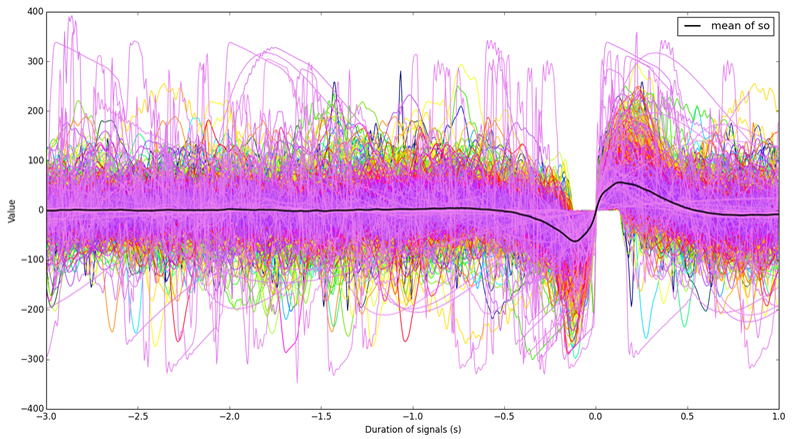
\includegraphics[width=0.7\textwidth]{EEG_oscillation.png}\\
	\vspace{15pt}
	\small Sleeping patient / 20 nights of EEG recordings\\
	\small Predict next slow wave
	}

\begin{frame}{EEG: Logistic Regression}
	
\end{frame}

  \begin{frame}\frametitle{Results}
    Nice table with SQN, SGD (no reg, L2), (Lasso,) Prox (L1) showing
    Obj. value in found optimum, CPU time, Iterations, F1 score of prediction model

    \begin{table}[t]
    \centering
      \begin{tabular}{r|c|c|c}
        \phantom 0 & \textbf{$F(\omega^*)$} & \textbf{Model Score} & \textbf{Cost}\\
      \hline \alert{No regularization}   &      & &  \\
        SGD   & $0.01$  & $96\%$  & $x$ sec, $y$ AP\\
        SQN   & $0.5$  & $96\%$  & $x$ sec, $y$ AP\\
        Prox   & $0.01$  & $96\%$  & $x$ sec, $y$ AP\\
      \hline \hline \alert{L1}        &    &   &  \\
      LASSO & $.71$  &  $55\%$ & blablabla \\
        Prox   & $0.01$  & $96\%$  & $x$ sec, $y$ AP\\
      \hline \hline \alert{L2}        &    &   &  \\
       SGD & $.71$  &  $55\%$ & blablabla \\
        SQN   & $0.01$  & $96\%$  & $x$ sec, $y$ AP\\
      \end{tabular}
    \end{table}
  \end{frame}

\section{Dictionary Learning}
\plain{Dictionary Learning\\
	\vspace{10pt}
	\alert{Can we recover the image?}
	\vspace{15pt}\\
	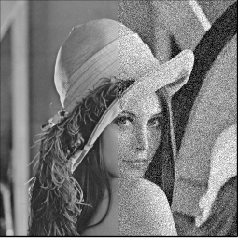
\includegraphics[width=0.4\textwidth]{lena_pic.jpg}\\
	\vspace{15pt}
	\small Image is partially destroyed\\
	\small Reconstruct image
}
\begin{frame}{Dictionary Learning}
	bla
\end{frame}

\section{Conclusion}

  \begin{frame}{Summary}
    \begin{center}\ccbysa\end{center}
  \end{frame}
  

  \plain{Questions?}

  \begin{frame}[allowframebreaks]\frametitle{Main References}

    \bibliography{refs}
    \bibliographystyle{abbrv}

  \end{frame}

\end{document}
